% The closed antipodal pair (co-active reading on the line) next to the opened pair
% (co-active reading inside the parallelogram).
% Compile from figures/ (the fonts resolve relative to the cwd): lualatex opening.tex,
% then pdftoppm -png -r 200 and autocrop to opening.png (see ../reproduce.sh).
\documentclass{article}
\usepackage[a4paper, landscape, margin=1cm]{geometry}
\pagestyle{empty}
\usepackage{fontspec}
\usepackage{xcolor}
\usepackage{amsmath}
\usepackage{tikz}
\setmainfont{Poppins}[
  Path = fonts/Poppins/,
  Extension = .ttf,
  UprightFont = *-Regular,
  BoldFont = *-Bold,
  ItalicFont = *-Italic,
  BoldItalicFont = *-BoldItalic
]
\definecolor{pivotalOrange}{HTML}{F15F22}
\definecolor{pivotalBlue}{HTML}{3A82B5}
\definecolor{pivotalNight}{HTML}{161616}
\definecolor{pivotalTaupe}{HTML}{818089}
\tikzset{
  feat/.style={-stealth, line width=2.4pt, pivotalBlue},
  axis/.style={-stealth, line width=1pt, pivotalTaupe!70},
  drop/.style={dotted, line width=1pt, pivotalTaupe},
  lbl/.style={font=\fontsize{20}{24}\selectfont},
  sm/.style={font=\fontsize{17}{20}\selectfont},
}
\begin{document}
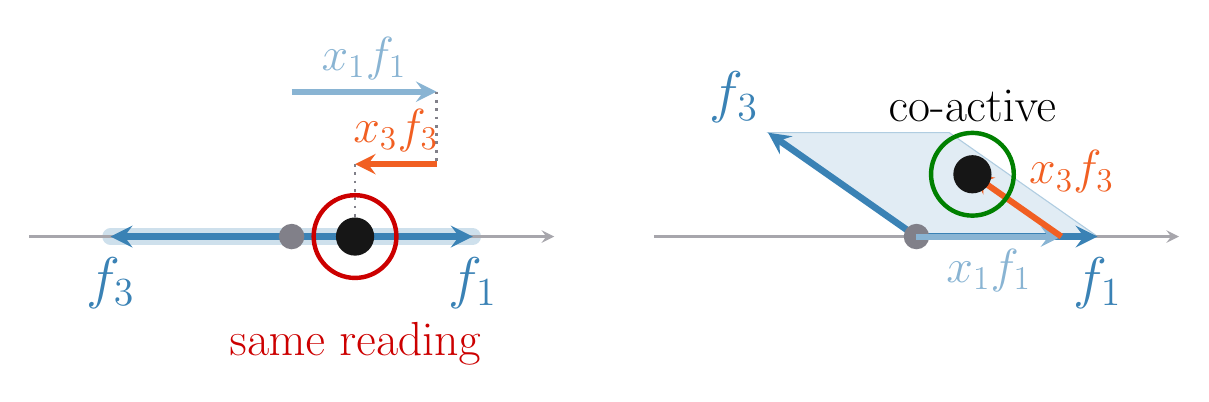
\begin{tikzpicture}[scale=2.3]
  % closed pair: one or two active features give the same point
  \draw[pivotalBlue!25, line width=6pt, line cap=round] (-1,0) -- (1,0);
  \draw[axis] (-1.45,0) -- (1.45,0);
  \draw[feat] (0,0) -- (1,0);
  \draw[feat] (0,0) -- (-1,0);
  \node[pivotalBlue, below, lbl] at (1,-0.06)  {$f_1$};
  \node[pivotalBlue, below, lbl] at (-1,-0.06) {$f_3$};
  \fill[pivotalTaupe] (0,0) circle (2pt);
  \draw[-stealth, line width=2.2pt, pivotalBlue!60] (0,0.8) -- (0.8,0.8)
    node[midway, above, sm] {$x_1 f_1$};
  \draw[drop] (0.8,0.8) -- (0.8,0.4);
  \draw[-stealth, line width=2.2pt, pivotalOrange] (0.8,0.4) -- (0.35,0.4)
    node[midway, above, sm] {$x_3 f_3$};
  \draw[drop] (0.35,0.4) -- (0.35,0);
  \fill[pivotalNight] (0.35,0) circle (3pt);
  \draw[red!80!black, line width=1.6pt] (0.35,0) circle (6.5pt);
  \node[below, sm, red!80!black] at (0.35,-0.42) {same reading};
  % open pair: the two inputs separate
  \begin{scope}[shift={(3.45,0)}]
    \fill[pivotalBlue!15] (0,0) -- (1,0) -- (0.181,0.574) -- (-0.819,0.574) -- cycle;
    \draw[pivotalBlue!40, thin] (0,0) -- (1,0) -- (0.181,0.574) -- (-0.819,0.574) -- cycle;
    \draw[axis] (-1.45,0) -- (1.45,0);
    \draw[feat] (0,0) -- (1,0);
    \draw[feat] (0,0) -- (145:1);
    \node[pivotalBlue, below, lbl] at (1,-0.06) {$f_1$};
    \node[pivotalBlue, above left, lbl] at (145:1) {$f_3$};
    \fill[pivotalTaupe] (0,0) circle (2pt);
    \draw[-stealth, line width=2.2pt, pivotalBlue!60] (0,0) -- (0.8,0)
      node[pos=0.5, below, sm] {$x_1 f_1$};
    \draw[-stealth, line width=2.2pt, pivotalOrange] (0.8,0) -- (0.309,0.344)
      node[midway, above right, sm] {$x_3 f_3$};
    \fill[pivotalNight] (0.309,0.344) circle (3pt);
    \draw[green!50!black, line width=1.6pt] (0.309,0.344) circle (6.5pt);
    \node[above, sm] at (0.309,0.58) {co-active};
  \end{scope}
\end{tikzpicture}
\end{document}
